%!TEX root = ../main.tex

\chapter{Introduction}\label{cha:introduction}

Deep Learning is a subclass of Machine Learning that has achieved state of the art results in a wide variety of domains.
They were originally proposed by McCulloch and Pitts in 1943 as a model for how the brain processes information \cite{McCulloch_Pitts_1943}.
In 1957, Rosenblatt created the Perceptron \cite{Rosenblatt_1957, Rosenblatt_1958}, however it was shown that it is impossible for these to learn the simple XOR function \cite{Minsky_Papert_1988}.
In the 1980's neural networks became popular again and Rumelhart, Hinton, and Williams wrote a famous paper outlining the backpropagation algorithm for training networks of neuron-like units \cite{Rumelhart_Hinton_Williams_1986}.
This algorithm remains at the core of all deep learning today.


\section{Neural Networks}\label{sec:neural_network_int}
The goal of a neural network is to approximate some function $f^*$.
Suppose there is a classifier $y=f^*(\bm{x})$ which maps inputs $\bm{x}$ to category $y$.
A neural network defines a mapping $\bm{y}=f(\bm{x}, \bm{\theta})$ and attempts to learn the values of parameter $\bm{\theta}$ that best approximate $f^*$.
The model is usually depicted as an acyclic graph which represents how several functions are composed together.
For example, three functions $f_1, f_2, f_3$ may be chained together such that $f(\bm{x}) = f_3(f_2(f_1(\bm{x})))$.

We refer to these networks as neural because they are inspired by the brain.
A neural network is a collection of connected nodes (simplified versions of  biological neurons).
A connection between two nodes (equivalent of a biological synapse) can transfer data from one node to the next.
The signal processed between two nodes is a real valued number, and the output is a non-linear function of the sum of its inputs.
Figure \ref{fig:neural_net} shows a simple neural network with 2 layers.

\begin{figure}[hbtp!]
    \centering
    \subfloat[A basic neural network]{\includestandalone[width = 0.5\textwidth]{./img/tikz/neural_net}\label{fig:neural_net}}
\end{figure}

In this diagram, we have 1 input layer, 1 hidden layer and 1 output layer and the network contains two functions $f_1, f_2$ that are chained together such that $f(\bm{x}) = f_2(f_1(\bm{x}))$.
The hidden layer $\bm{h}$ is given by:

\begin{equation}
    \bm{h} = f_1(\bm{x}; \bm{W_1}, \bm{b_1}) = g(\bm{W_1}^\top \cdot \bm{x} + \bm{b_1})
    \label{eq:hidden_layer}
\end{equation}
.
The output layer $\bm{y}$ is given by:

\begin{equation}
    \bm{y} = f_2(\bm{h}; \bm{W_2}, \bm{b_2}) = g(\bm{W_2}^\top \cdot \bm{h} + \bm{b_2})
    \label{eq:output_layer}
\end{equation}

Where $g$ is a non-linear activation function , $\bm{W_1}, \bm{W_2}$ are weight matrices and $\bm{b_1}, \bm{b_2}$ are bias vectors.
Thus each node is non-linear function of the sum of its inputs, as mentioned earlier.

A way of evaluating the neural network is now needed.
The MSE loss function over the training set $\mathbb{X}$ is defined as:

\begin{equation}
    J(\bm{\theta}) = \frac{1}{4} \sum_{\bm{x} \in \mathbb{X}} (f^*(\bm{x}) - f(\bm{x}; \bm{\theta}))^2
    \label{mse_loss_function}
\end{equation}

Where $\bm{\theta}$ represents all learnable parameters $\bm{W_1}, \bm{W_2}, \bm{b_1}, \bm{b_2}$.
Now $J(\bm{\theta})$ must be minimised with respect to $\bm{W_1}, \bm{W_2}, \bm{b_1}, \bm{b_2}$.

% TODO discuss activation functions
\begin{figure}[hbtp!]
    \centering
    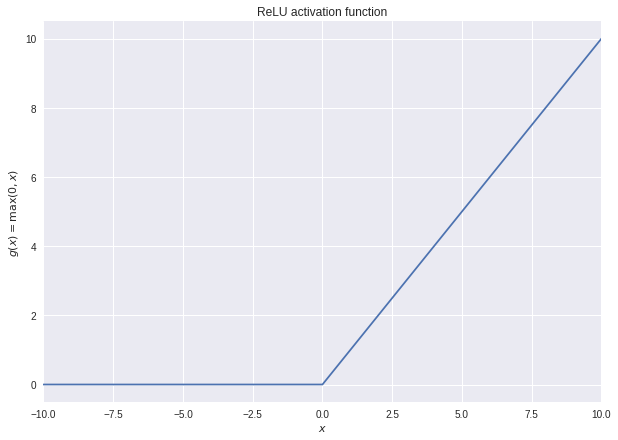
\includegraphics[width=0.45\textwidth]{./img/ReLU.png}
    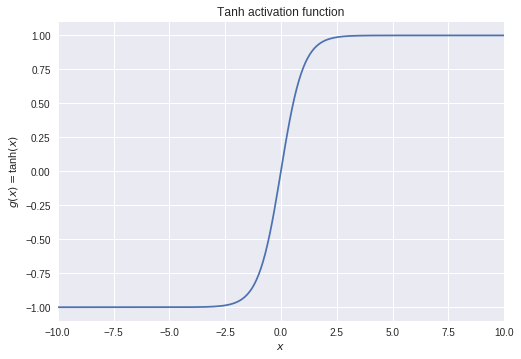
\includegraphics[width=0.45\textwidth]{./img/tanh.png}
    \caption{The Rectified Linear Unit (ReLU) and $\tanh$ activation functions}
    \label{fig:ReLU_tanh}
\end{figure}



\section{Problem Description}\label{sec:problem_description_int}
%TODO introduction to deep learning in healthcare
Detecting cancers in medical images is an important task in modern health care.

\subsection{PET Scans}\label{subsec:pet_scan_int}
Positron Emission Tomography (PET) scans are used to produce 3 Dimensional images of the human body and are often combined with CT scans (called PET-CT) or MRI scans (PET-MRI) in order to increase the level of detail.
PET scans are particularly useful because they describe how certain parts of the body are functioning in addition to their physical appearance.
PET scans are most commonly used for investigating confirmed cases of cancer to determine how far the cancer has spread and how well it's responding to treatment \cite{Radiology_ACR, PET_scan}.
The procedure is as follows:

\begin{itemize}
    \item A radioactive tracer (often glucose based) is introduced to the patient either by injection into the bloodstream, swallowing or inhalation as a gas.
    \item For a glucose based tracer, cells in the body with a high metabolic rate will accumulate the tracer.
    \item The tracer gives off a small amount of energy in the form of gamma rays which is detected by the scanner.
    \item A computer then produces a 3D image in which hotspots indicate a large amount of tracer accumulation and therefore a high level of metabolic activity.
\end{itemize}

% TODO include some example pet scan images

\subsection{Current Data}\label{subsec:current_data_intro}

% %TODO explain The Data
% %TODO explain Ground Truth and what we hope to achieve


\section{Structure}\label{sec:structure}

\begin{itemize}
    \item In Chapter \ref{cha:literature} an overview of previous literature regarding Deep Learning is given.
    \item In Chapter \ref{cha:initial_results} an outline of current work and potential future developments is outlined.
\end{itemize}